\chapter{Rivers: Applicações Reais}
\label{cha:applications}

\section{Appx - Appengine eXtensions}
\label{sec:appx}

\emph{Appx} \cite{docs:drborges:appx} é um conjunto de extensões da plataforma \emph{Appengine} da Google \cite{docs:google:appengine} para o runtime da linguagem Go que oferece uma solução similar à Object Relational Mapping \cite{article:scott:orm} para modelagem da camada de domínio de aplicações que utilizam a solução de \emph{NoSQL} \cite{article:fowler:nosql} Datastore \cite{docs:google:datastore} da plataforma. Rivers foi utilizado para dar suporte à \emph{Continuous Querying Over Data Stream} \cite{paper:badu:continuous_querying}, permitindo que grandes conjuntos de dados possam ser continuamente buscados da base de dados em batches via paginação e processados assincronamente como um stream de entidades Datastore em poucas linhas de código.

Processar um grande conjunto de dados aplicando filtros, mapeamentos e realizando a paginação dos resultados é relativamente complexo quando se utilizando apenas as APIs nativas do Datastore. Desenvolvedores precisam explicitamente implementar a paginação contínua dos dados através da manipulação de cursores de busca, realizar tratamento de possíveis erros de execução além de implementar a lógica de processamento dos dados, sendo necessário várias linhas de código para se obter o resultado final levando a uma solução difícil de manter e muita duplicação de código quando esse processamento deve ser aplicado à diferentes entidades da base de dados. A figura \ref{code:datastore:pagination} mostra a implementação de um agendador de reuniões que envia email, sms e atualiza o calendário de cada empregado de uma empresa cujo título seja \emph{Manager} ou \emph{Director} com as informações da reunião. Devido a uma limitação do Datastore, é possível processar no máximo 1000 entidades por vez, sendo necessário realizar a paginação contínua dos dados até que todos eles sejam processados. Grande parte desta implementação não possui relação direta com a lógica necessária para o agendamento da reunião mas sim com a paginação dos dados.

\begin{figure}[H]
  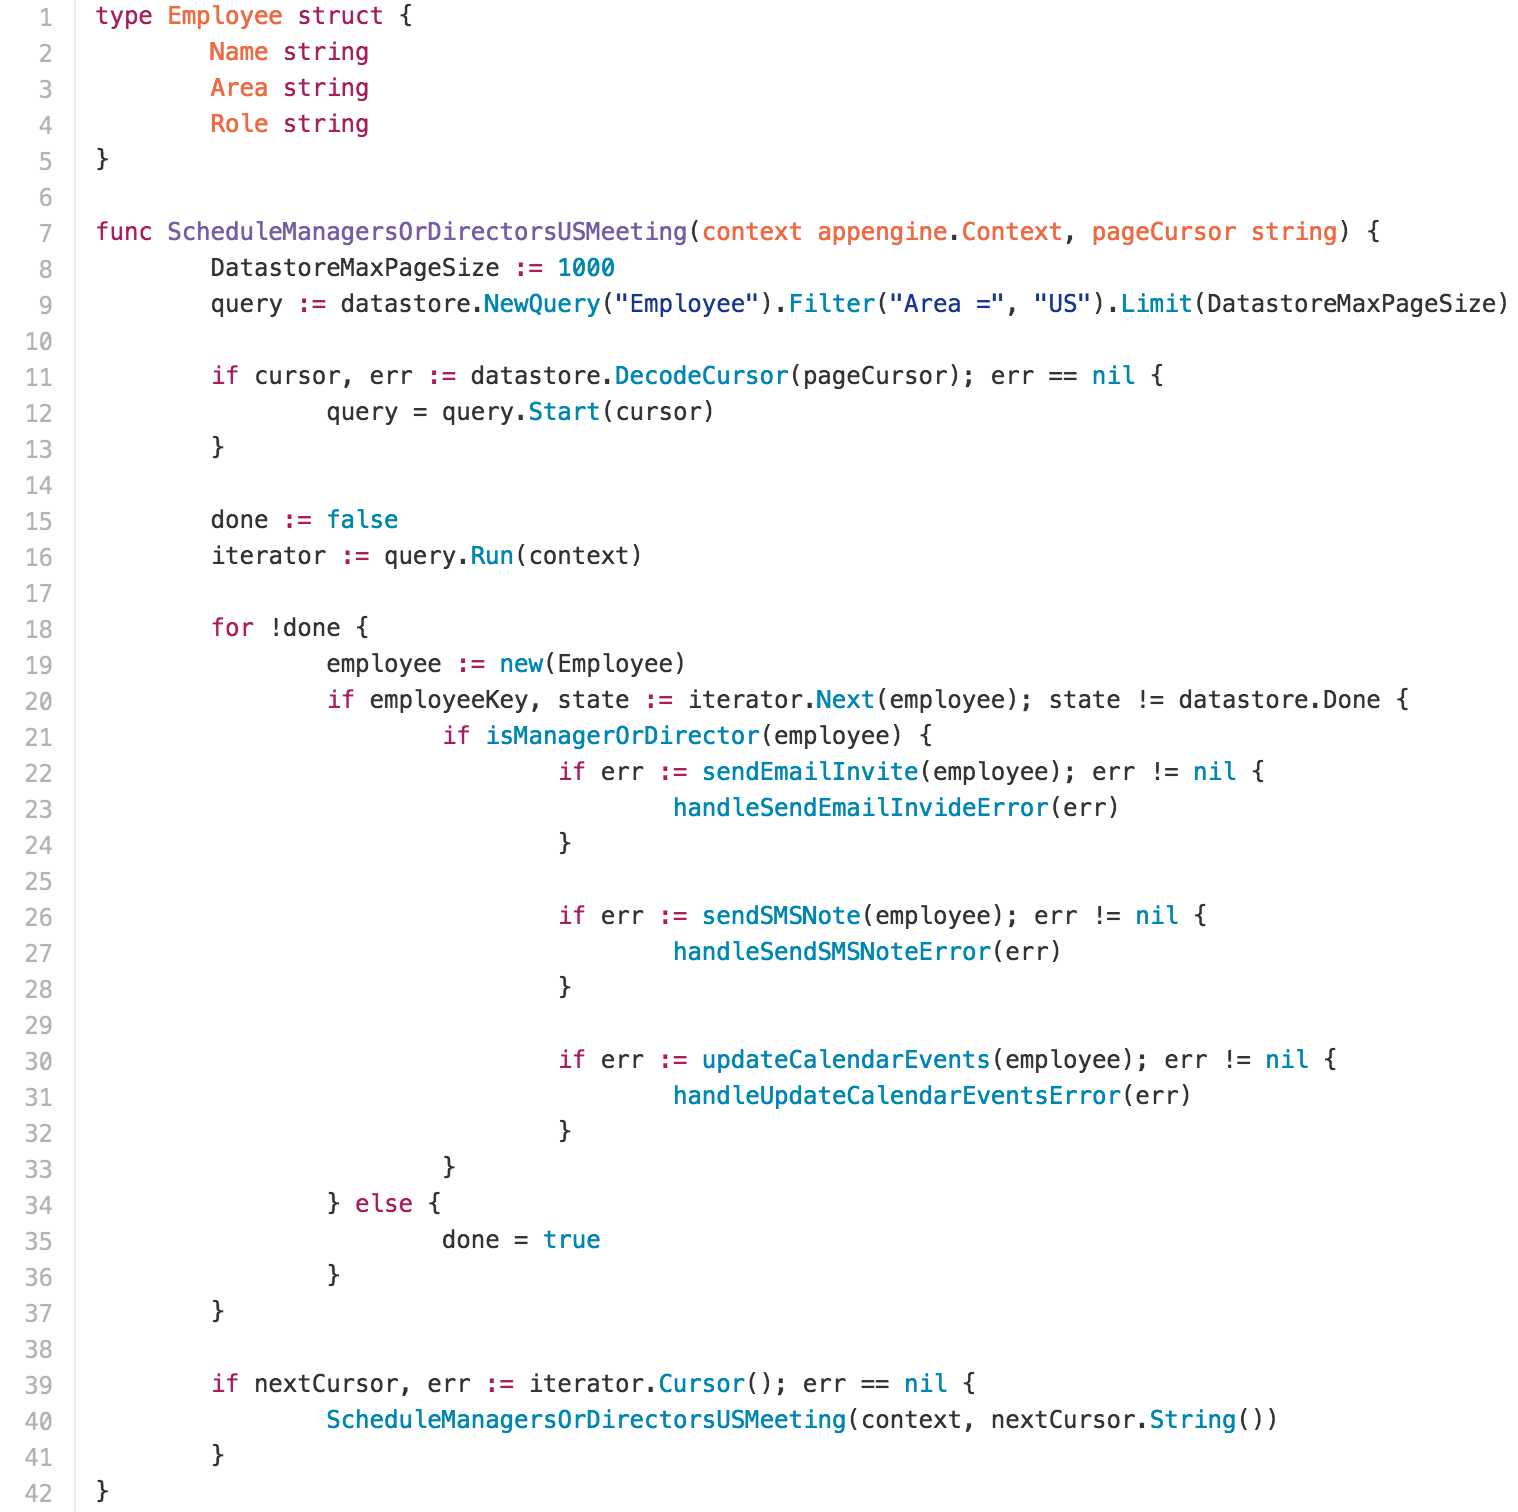
\includegraphics[width=1\textwidth]{datastore_pagination}
  \centering
  \caption{Exemplo de uso da API nativa do Datastore.}
  \label{code:datastore:pagination}
\end{figure}

Appx utiliza Rivers para reduzir grande parte desta complexidade sendo necessárias poucas linhas de código para se obter o mesmo resultado do exemplo anterior. A figura \ref{code:appx:stream} mostra como podemos reescrever este mesmo caso de uso utilizando a API de streamming de Appx. Devido à arquitetura extensível de Rivers sua integração com Appx é relativamente simples, sendo necessário que Appx apenas implemente a interface \emph{stream.Producer} de Rivers que encapsula a execução da query, tratamento de erros e a paginação contínua dos resultados emitindo cada entidade datastore que satisfaz a query em um \emph{stream.Readable} ao qual operações como \emph{Filter}, \emph{Each}, \emph{Map} e \emph{Reduce} podem ser aplicadas formando um pipeline de processamento de entidades \emph{Datastore}. Desta maneira o resultado final não é somente mais legível mas como também fácil de manter e alterações na lógica de processamento é tão simples como adicionar ou remover filters, mappers, etc. 

\begin{figure}[H]
  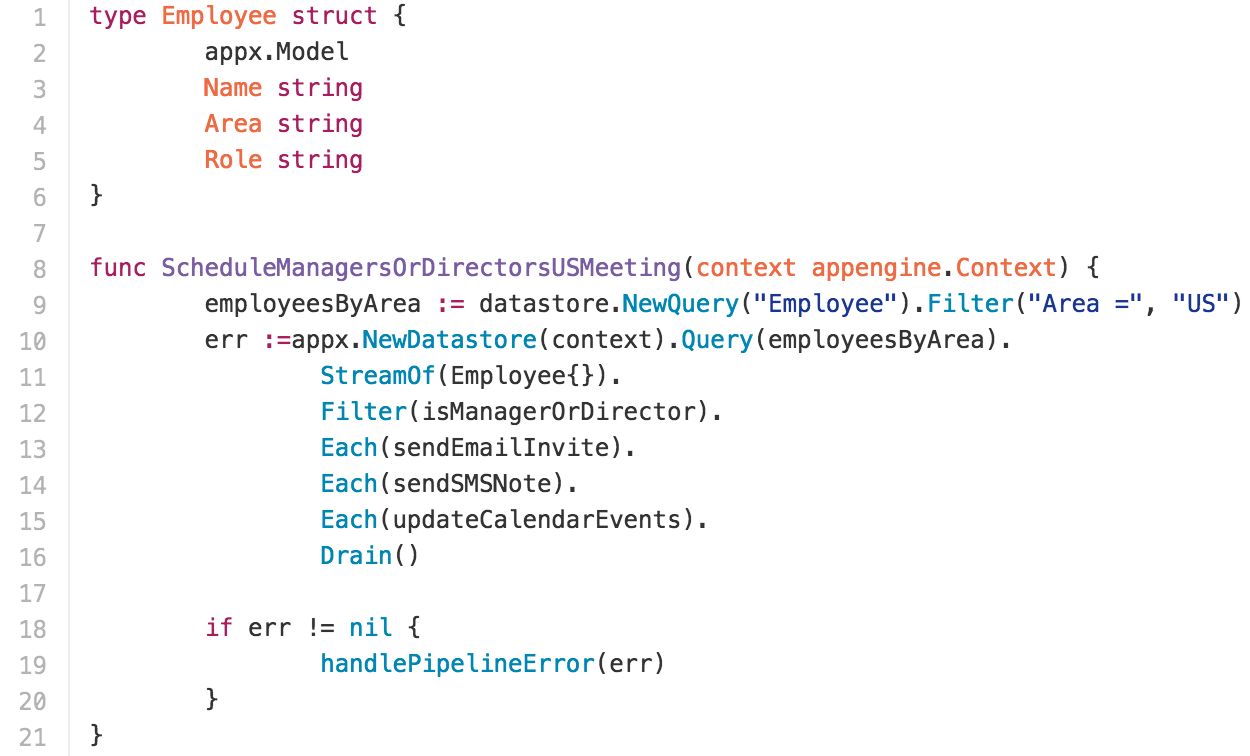
\includegraphics[width=1\textwidth]{appx_stream}
  \centering
  \caption{Exemplo de uso da API de streamming do framework Appx.}
  \label{code:appx:stream}
\end{figure}

\section{Web Scrapping}
\label{sec:web_scrapping}

Web Scraping \cite{article:webharvy:scrapping} é uma solução simples, barata e eficaz para coleta e extração de dados na web e frequentemente são aplicados em conjunto com \emph{Web Crawlers} \cite{article:howstuffworks:web_crawler}, sistemas responsáveis por automatizar a busca e descoberta da informação, basicamente acessando documentos web através de \emph{URLs}, coletando e visitando cada URL no documento retornado aplicando este processo recursivamente até que uma determinada condição de parada seja satisfeita, afim de extrair e agregar determinados tipos de informação presentes em cada documento.

Este processo de crawling por envolver altos níveis de tráfego de rede pode vir a ser muito custoso e a possibilidade de paralelizar partes do processo pode ajudar a reduzir este custo. Rivers pode ser utilizado na implementação de pipelines com foco em Web Crawling e Scrapping, aonde cada crawler implementa a interface \emph{stream.Producer} com uma lógica específica responsável por "caminhar" a web seguindo determinadas regras específicas do crawler passando cada documento encontrado ao próximo estágio do pipeline que implementa a interface \emph{stream.Transformer} responsável por extrair as informações necessárias do documento implementando a função de scrapping. A imagen \ref{code:crawler} mostra um exemplo de Crawler utilizado como \emph{stream.Producer} em um pipeline Rivers responsável por extrair URLs de documentos HTML com a listagem de gastos públicos das cidades do Rio Grande do Sul disponíveis no \cite{portal_transparencia}, passando cada URL ao estágio seguinte do pipeline que implementa um scrapper \ref{code:scrapper} que dado uma URL o documento correspondente é recuperado via HTTP e as informações de gastos extraídas e coletadas em um dicionário chave-valor aonde a chave representa a área correspondente ao gasto como por exemplo educação ou saúde, e seu valor o total investido nesta área. A figura \ref{code:scrapping_example} mostra o uso do Crawler e Scrapper em um pipeline Rivers com paralelização ativa, podendo processar até 510 URLs em paralelo que é o número total de cidades a serem processadas e representa a capacidade máxima de produção do pipeline especificado pelo Crawler na linha 25.

\begin{figure}[H]
  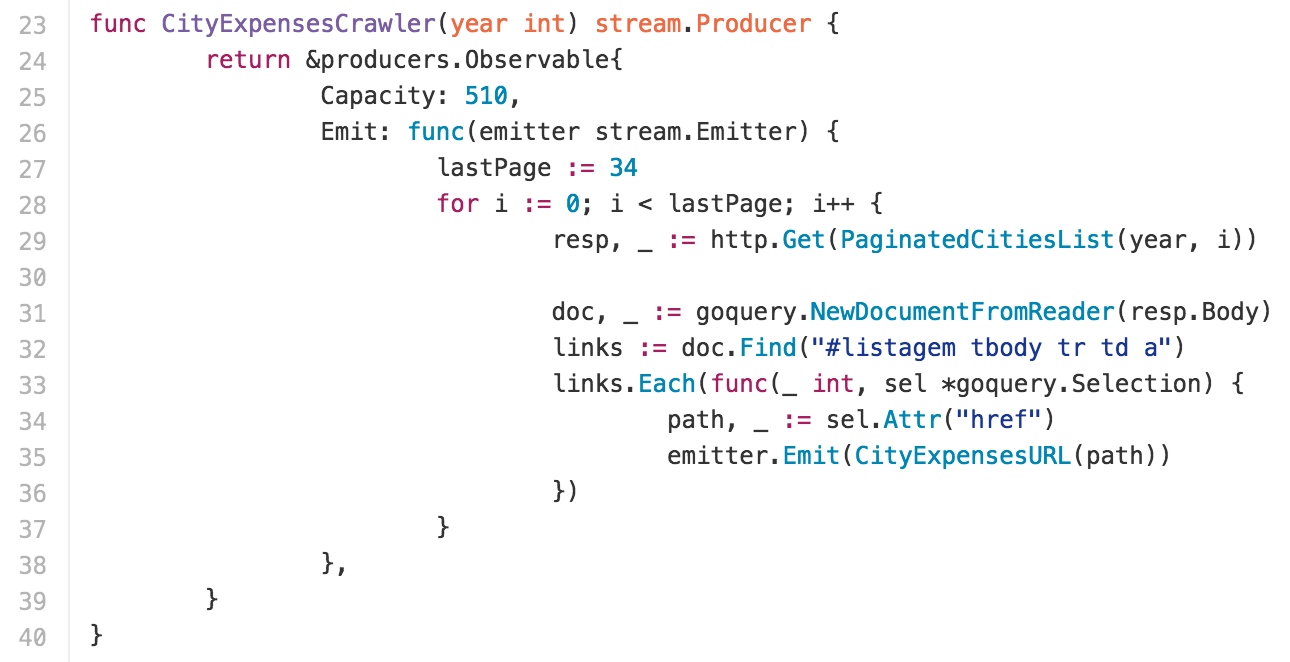
\includegraphics[width=1\textwidth]{crawler}
  \centering
  \caption{Exemplo de um Crawler que implementa a interface stream.Producer.}
  \label{code:crawler}
\end{figure}

\begin{figure}[H]
  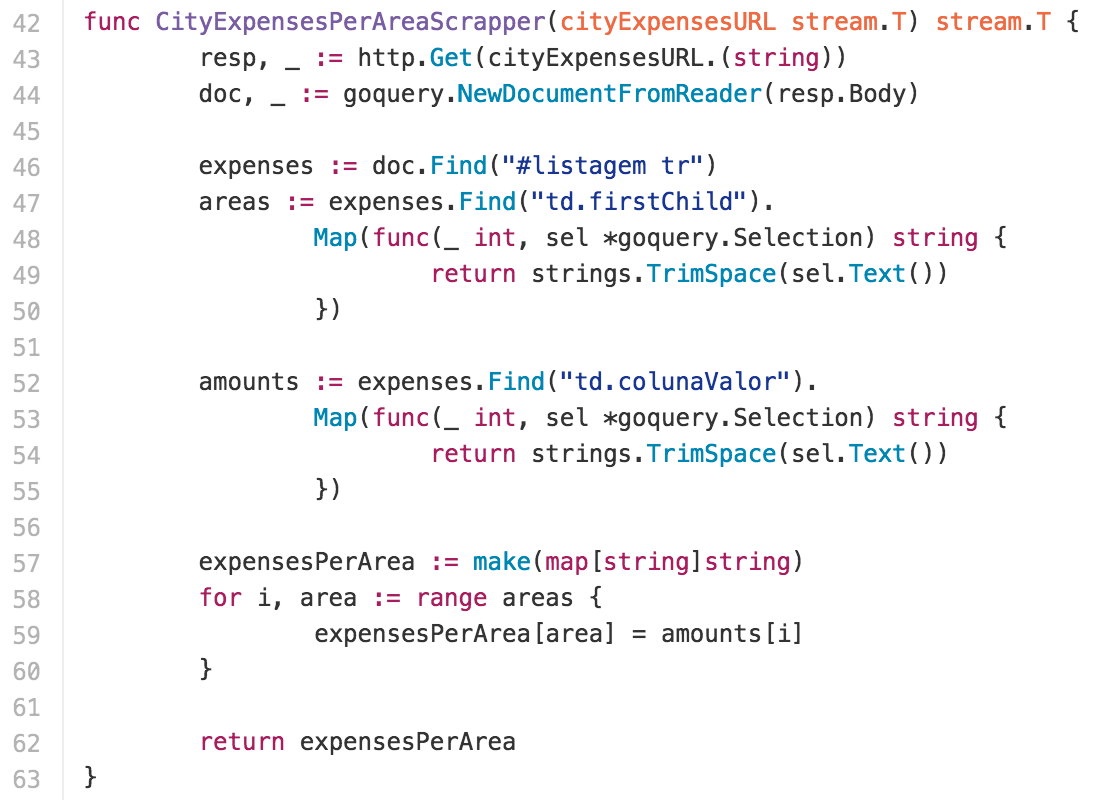
\includegraphics[width=1\textwidth]{scrapper}
  \centering
  \caption{Exemplo de um Scrapper que implementa a interface stream.Transformer.}
  \label{code:scrapper}
\end{figure}

\begin{figure}[H]
  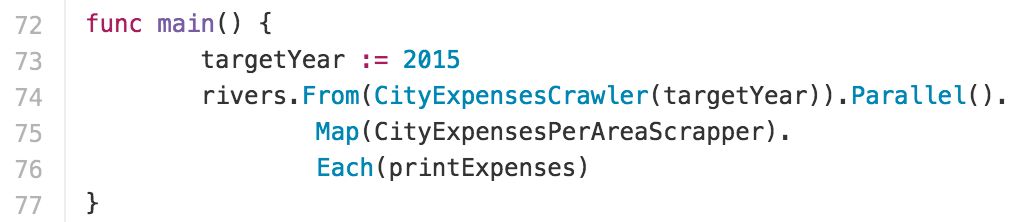
\includegraphics[width=1\textwidth]{scrapping_example}
  \centering
  \caption{Exemplo de uso do Crawler e Scrapper em um pipeline Rivers.}
  \label{code:scrapping_example}
\end{figure}